%!TEX root = ../Thesis.tex
\label{chapter:introduction}
Privacy and security have been the center of attention when it comes to technological innovation. Both privacy and security of the user are important factors for technology to be accepted by wide population. However, some technologies do not put much effort into privacy and security. In this chapter, we discuss what wearable devices are and their significance in the 21st century. We also briefly define what physiological data is and the benefits of physiological data in health, sports and training, and marketing and advertisement. In the next chapter, we will take a look at security and privacy issues surrounding wearable devices with some examples. 

\paragraph{Wearable Devices}
Wearable devices can be worn or mated with human skin to continuously and closely monitor an individual’s activities, without interrupting or limiting the user’s motions \cite{gao_fully_2016}. These devices can perform sophisticated tasks such as biofeedback and tracking of physiological data \cite{noauthor_wearable_nodate}.

\paragraph{Growth} The steady growth of fitness and health-conscious consumers has driven the innovation in wearable devices. The wearable industry is estimated to be worth \$19.63 billion \cite{noauthor_wearable_market_nodate}. The shipments of global wearable devices are expected to grow by 55\% by 2022 \cite{WearableStudy} to worth of \$57.63 billion \cite{noauthor_wearable_market_nodate}. The most popular of wearable devices are smart watches and fitness trackers as visualized in Figure \ref{fig:forecast_of_wearable_devices}.

\begin{figure}
    \centering
    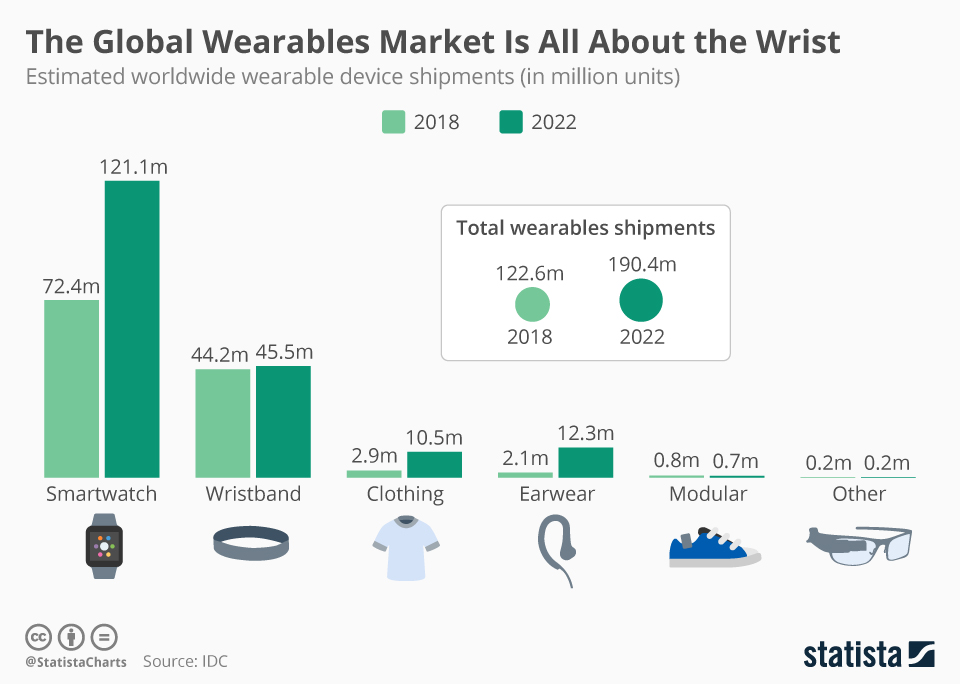
\includegraphics[width=100mm]{wearable_device_forecast.jpg}
    \caption{Forecast of Wearable Devices 2018-2022 \cite{WearableStudy}.}
    \label{fig:forecast_of_wearable_devices}
\end{figure}


\paragraph{Fitness Trackers}
Fitness trackers are wearable devices that are focused on monitoring physical activities for healthcare. Fitness trackers are designed to be worn all day and track physical activities of the users. Table \ref{tab:data_wearable_devices} shows an overview of data managed by the fitness trackers \cite{mendoza_assessment_2018}. While the range of physiological data collected by the fitness trackers is limited measuring floors climbed, steps, heart rate, and sleep quality, the innovation in semiconductor technology in recent years has enabled the development of sensors. The development of better sensors which can measure other vital physiological data like Electrocardiogram (ECG) and Electrodermal activity (EDA) are now closer to realization in everyday product. \cite{haghi_wearable_2017}. 

\begin{center}
\begin{tabular}{ |c|c|c| }
\hline
\textbf{Data Type} & \textbf{Basic Attributes} & \textbf{Additional Attribute} \\
\hline
\hline
\multirow{5}{8em}{Personal data} & Gender & Food log \\ 
& Age & Water log \\ 
& Date of Birth & Location \\ 
& Height & Profile photos \\ 
& Weight & Alarms \\ 
\hline
\multirow{1}{8em}{Contact info} & Email & Contacts \\
\hline
\multirow{4}{8em}{Activity Data} & Steps &  \\
& Floors & \\
& Heart rate & \\
& Sleep quality & \\
\hline
\multirow{3}{8em}{Device info} & Battery level & \\
& Sync time & \\
& App info & \\
\hline
\end{tabular}
\captionof{table}{Data collected by fitness trackers \cite{mendoza_assessment_2018}.}
\label{tab:data_wearable_devices}
\end{center}

 \paragraph{Physiological Data} Physiology is a discipline of biology which deals with the study of the functioning of living organisms, animals or plants, and of the functioning of their constituent tissues or cells \cite{scheer_physiology_nodate}. Direct measure of physiological changes in users can provide insight into a user's cognitive and emotional state \cite{benbasat_incorporating_nodate}. These physiological measures include Electroencephalogram (EEG) alpha and beta, EDA, heart rate, and heart rate variability which have been found to relate to the ability of cogitative learning (how a person processes and reasons the information) \cite{leger_neurophysiological_2014}.
 
\paragraph{Health Benefits} Having access to users physiological data has many health benefits. It can help diagnose several medical conditions including multiple sclerosis (MS), a multifactorial demyelinating disease of the central nervous system \cite{sparaco_role_2018}, atrial fibrillation (AFib), a heart condition \cite{nemati_monitoring_2016}, sleep apnea, hypertension \cite{tison_geoffrey_h_abstract_2017} and many more.

\paragraph{Sports and Training} The study of the effect of exercise on physiology can be traced back to 1877, in the book \textit{The Principles and Practices of Medicine}. Author and pioneer physician-scientist Austin Flint, Jr., M.D. discussed the influence of posture and exercise on pulse rate and influence of activity on respiration \cite{mcardle_essentials_2006}. Since then, researchers have tried to understand the consequences of exercise and training on the cardiovascular system using heart rate variability (HRV), aortic blood pressure variability (BPV) etc \cite{aubert_heart_2003}. The study conducted by \citeauthor{vesterinen_individual_2016}, the subjects undergoing HRV-guided training showed significant improvement in fitness over the predefined training \cite{vesterinen_individual_2016}. Thus, it is clear that fitness trackers will have a significant role to play in sports and training.

\paragraph{Marketing and Advertisement} The relation of physiological response to the television commercials was first studied by \citeauthor{522761019710201} by measuring EEG of the subject \cite{522761019710201}. The study was criticized as it failed to explain what was being measured in marketing terms. For example, marketing scholars criticized that the ratio between alpha and beta waves was used to indicate arousal in the subjects, however, it wasn't clear if this was due to the effective response due to the advertisement being shown or a complex cognitive state due to internal physiology of the body \cite{1907543419840330}. The advances in neuroimaging in the past few decades have again sparked interest in understanding consumer behavior. Hence giving birth to a new communication marketing field called \textit{neuromarketing} \cite{ait_hammou_contributions_2013}. Researchers are now trying to understand how emotions induced by advertisements influence the EDA and the ECG. \cite{baraybar-fernandez_evaluation_2017}. Though there are no conclusive results yet regarding the relation between advertisements and physiological data like EDA and ECG. The popularity of smartwatches and fitness trackers and their ability to gather accurate physiological data round the clock would attract many neuromarketing researcher's attention.


\section{Structure of this Thesis}
The thesis is structured as follows.
\paragraph{Chapter 2} We give an overview of our reason and inspiration behind this study. We focus on the security and privacy issues surrounding the fitness trackers and lay out our goals, methodology, and objective for the thesis.

\paragraph{Chapter 3} In this chapter we familiarize with the ECG and the EDA physiological signals and understand their importance in our study. We also learn the best practices for collecting and quantifying ECG and EDA.

\paragraph{Chapter 4} We review the related studies and research conducted in the past. We learn about the methodologies of the studies done relating to our study and summarize them.

\paragraph{Chapter 5} In this chapter we lay out the methodology of collecting physiological data used in this study. We discuss our choice of device, BITalino, for recording physiological signals and the reason why we choose to use it. We discuss the anatomy of BITalino and explain the best practices to record the physiological signals using the BITalino. We further discuss the challenges faced while recording physiological signals and how we countered them. We conclude with the experimental setup used in this study.

\paragraph{Chapter 6} We evaluate the demographics and self-assessment of emotions while watching the movies by the subjects. We then explain the machine learning and deep learning models we used in our analysis, their implementation and discuss the results.

\paragraph{Chapter 7} We conclude the thesis with a review of our study. We scrutinize our results and layout the privacy implication of wearable devices collecting vital physiological data. We end with laying out the possible improvements that can be done to improve the results. 